% \chapter{Discussion}
% \label{cha:discussion}
\chapter{Conclusion}
\label{cha:conclusion}

The focus of this report have been two-part. In the first part, methods for
vibration-based identification of nonlinearities have been explored and
validated. No assumption of the type of nonlinearity have been made, thus the
models works equally well for boundary, geometric, etc. types of nonlinearities.
Only stiffness have been treated; in theory the methods works just as well for
damping, but in practice damping is much harder due to the much smaller
magnitude and successful identification is still hard to obtain \textbf{Put ref
  på.}. Another subject that been neglected, is identification with noisy
signals. To get good estimates from noisy signals is difficult and more research
have to be done in order to get consistent results.

In the second part, methods for investigating the behaviour of identified
nonlinear systems are treated. On the successful identification in part one, a
model is built and used for determine stability, bifurcations and internal
resonances. Where the methods in the first part requires some understanding and
knowledge about nonlinear system in order to obtain a good identification, the
methods here are easier to use and do not require as much knowledge (that said,
implementation wise they cannot be said to be easier).

One substantial lack in connecting the two parts, is the need to create a model
after identification is done. Current research are focused on eliminating this
step, and use the state space system identified by FNSI directly by the
numerical methods of the second part\autocite{gourc2016a}. Numerically this is
easy when both the FNSI and HB methods are implemented, but as shown in section
\ref{sec:fnsi-estimation-error}, the FNSI method introduce spurious numerical
artefacts, and as long as these artefacts are present, the state space
formulation cannot be used directly. Preventing artefacts in the FNSI method
will be a big step forward in the seamless integration of the two methodologies.
Figure \ref{fig:fnsi_hb} shows the methodology.

\begin{figure}[!ht]
  \centering
  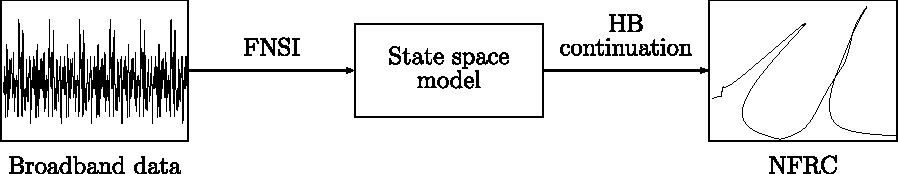
\includegraphics[width=0.7\linewidth]{discussion/fnsi_hb.pdf}
  \caption{FNSI-HB continuation procedure}
  \label{fig:fnsi_hb}
 \end{figure}



%%% Local Variables:
%%% mode: latex
%%% TeX-master: "../report"
%%% End:
